%! Author = evandro
%! Date = 13/02/21

% Preamble
\providecommand{\report}{..}
\documentclass[../main.tex]{subfiles}

% Packages

% Document
\begin{document}
    \chapter{Descrizione del modello}\label{ch:descrizione-del-modello}
    In questo capitolo si descrive il modello sviluppato.


    \section{Formalizzazione del problema}\label{sec:formalizzazione-del-problema}
    Dalla descrizione del problema ho deciso di modellarlo come un modello multi-classe con tre stazioni di coda.
    Ogni stazione di coda rappresenta un diverso componente dell' architettura \textit{three tier}.
    Le stazioni di coda sono disposte in sequenza: stazione del \textit{web server}, la stazione del \textit{application server} e infine la stazione del \textit{database}
    In particolare, ogni stazione è caratterizzata da una coda limitata e dal numero di repliche.

    \centering
    \begin{figure}[H]
        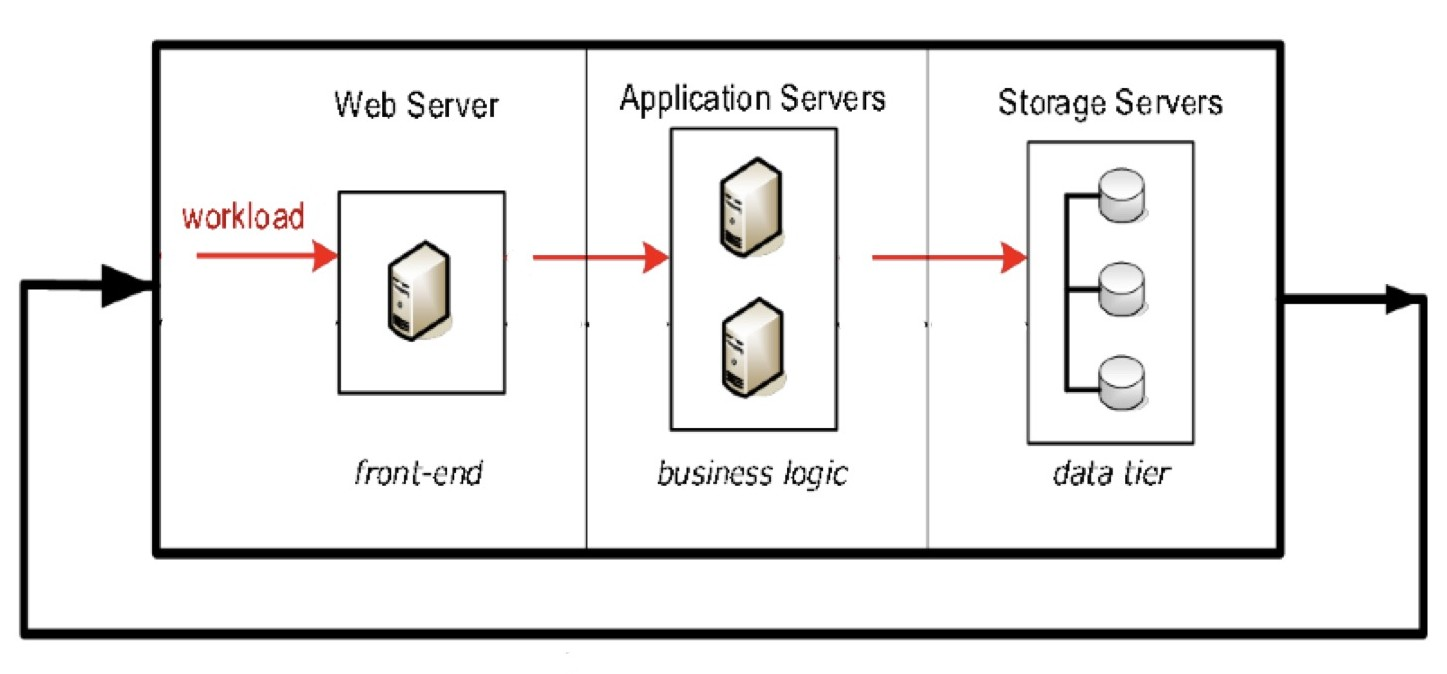
\includegraphics[scale = 0.3]{assets/three_tier}\\
        \caption[\textit{Architettura} del modello]{architetture del modello di alto livello.}
        \label{fig:architettura-del-modello}
    \end{figure}


    \section{Le classi}\label{sec:le-classi}
    I \textit{jobs} che circolano nel sistema sonno stati identificati con tre diverse classi: tutti i \textit{jobs} che appartengono alla stessa classe, sono caratterizzati dalle stesse proprietà.


    \section{Le componenti del modello}\label{sec:le-componenti-del-modello}


    \section{L'architettura del modello completo}\label{sec:l'architettura-del-modello-completo}


\end{document}